%
\section{Device drivers}
\label{sec:device-drivers}

A device driver is a small piece of software that tells the operating system and other software how to communicate with a piece of hardware.~\cite{ddrivers}

When the kernel recognizes that a certain action were requested to a device, it calls an appropriate function from the driver, and transfers the process control from the user to the driver function.
After the driver function ends its execution, it gives the
control back to the user space process.

The device driver provides the following characteristics:

\begin{enumerate}[label=\roman*.]
\item A set of functions to communicate with the hardware
device, and a standardized kernel interface; 
\item It shoud be an autonomous component, able to be
dynamically added to and removed from the OS;
\item Data flux control between the user space program and
device;
\item A user defined section, so the device driver can be
visible as a node in the /dev, for the OS.
\end{enumerate}

\begin{figure}[htb!]
\centering
    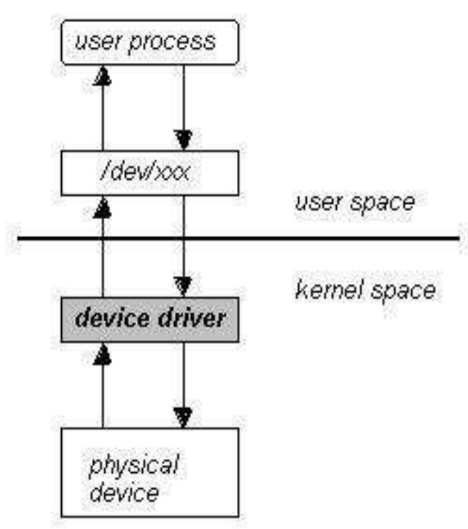
\includegraphics[width=0.35\columnwidth]{./img/ddrivers-char.png}
  \caption{Example of the usage of a device driver (withdrawn from~\cite{ddrivers-slides})}%
\label{fig:ddrivers-char}
\end{figure}

Character device drivers and Block device drivers are the two of the most important device drivers.
Block device drivers are accessed by the user space program by a system buffer that works like a data cache. There's no need for management or allocation routines as the system transfers the data from/to the device.
Character device drivers communicate directly with the user space program, so no buffer is required.~\cite{ddrivers-slides}


\subsection{Kernel mode vs Application}
\paragraph{\textbf{How an application can access to module services?}}

\begin{enumerate}[label=\roman*.]
%
\item When one of the kernel functions associate to the driver is called, the function \texttt{$module\_init()$} calls the function \texttt{$register\_capability()$} to register the driver services on kernel - on character drivers this is done by \texttt{$chrdev\_region()$} and \texttt{$alloc\_chrdev\_region()$}.
\item The function \texttt{$register\_capability()$} saves a pointer to an argument in the intern data struct \texttt{"$capabilities[]$"}
\item The system defines a protocol of how the application
will have access to \texttt{$capabilities[]$} by system calls
\item When the driver is no more necessary, the module
can be unregistered from kernel, freeing the entry on
\texttt{$capabilities[]$} using the function \texttt{$module\_exit()$}
%
\end{enumerate}

\texttt{The modules run on kernel space, while the applications run on user space.}

\begin{figure}[htb!]
\centering
    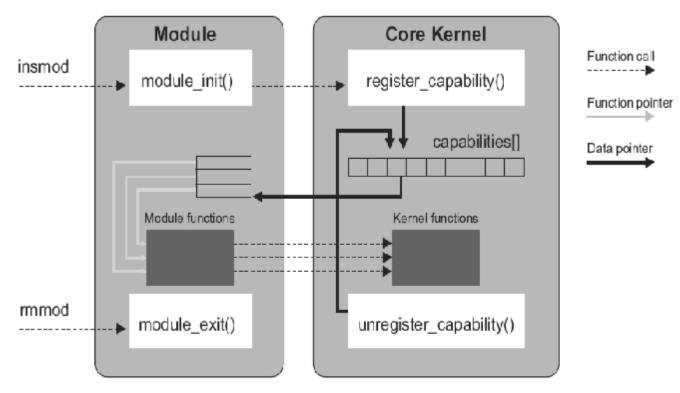
\includegraphics[width=0.6\columnwidth]{./img/ddrivers-kernel.png}
  \caption{Application accessing to module services (withdrawn from~\cite{ddrivers-slides})}%
\label{fig:ddrivers-kernel}
\end{figure}

Linux kernel offers a set of functions to the user space for the interaction with hardware.
Linux represents and manages a byte sequence using files.
Almost all devices are represented by a sequence of bytes, so linux also represents the I/O devices as special files called nodes with entries in \texttt{/dev} directory.

In the kernel space, Linux offers a set of functions that interact directly with the hardware and allows data transfer between kernel space and user space.

Normally, for each function in user space there is a matching function in the kernel space allowing data transfer between kernel and user space.

\begin{figure}[htb!]
\centering
    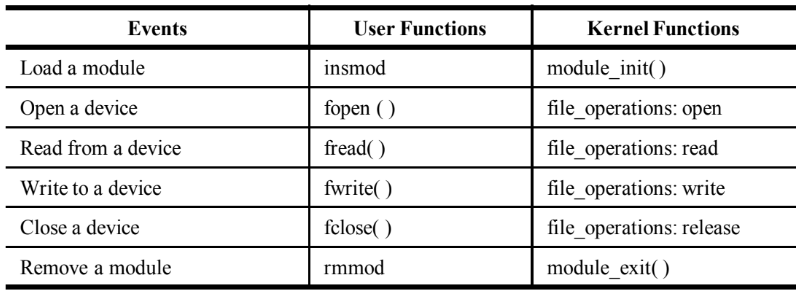
\includegraphics[width=0.75\columnwidth]{./img/ddrivers-events-ex.png}
  \caption{Examples of drivers event and corresponding interface functions between kernel space and user space (withdrawn from~\cite{ddrivers-slides})}%
\label{fig:ddrivers-events-ex}
\end{figure}

To associate the normal files to the kernel mode, the linux
system uses the major number and the minor number:

\texttt{Major number} is normally used by linux system to map \gls{io} requests to driver code. 
By other words, identifies the driver associated to the device.


\texttt{Minor number} is dedicated to internal use and it is used by kernel to determine exactly which device was referenced. 
Depending on the way the driver was coded,
this number can have a direct meaning, as a device counter, or it can be a simple driver iterator on the local devices array on kernel.

To do the association, it should be created a file or node in \texttt{/dev} directory, (calling \texttt{mknod} as root user) that will be used to access the driver

%%% Local Variables:
%%% mode: latex
%%% TeX-master: "../../../dissertation"
%%% End:
